\subsection{Les conditions initiales}

Les relations nous permettant d'apporter des conditions satisfaisantes au
système sont données par les formules de Frank, King et Raine avec $P =
P_\textrm{gaz}$ et $\kappa_\textrm{ff} \gg \kappa_\textrm{e}$
\cite{F_K_R-1985}. Ces conditions en $\Sigma$ et $T$ sont suffisamment petites
pour ne pas influencer le système lors de son évolution. $\dot{M}$ est pris
très petit devant  le taux $\dot{M_{0}}$ imposé au système : 

\begin{equation}
	\dot{M} = 1\ 10^{-1 }\dot{M_{0}}
\end{equation} 

\begin{equation}
	T = 1.4 \times 10^{4} \alpha^{- \frac{1}{5}} \left[ \frac{\dot{M}}{10^{16} \mathrm{g.s}^{-1}} \right]^{\frac{3}{10}} \left[ \frac{M}{M_\odot}\right]^{\frac{1}{4}} \left[ \frac{r}{10^{10}\mathrm{cm}}\right]^{- \frac{3}{4}} f^{\frac{3}{10}} \mathrm{K} 
\end{equation}

\begin{align}
	\Sigma = 5.2 \alpha^{- \frac{4}{5}} \left[ \frac{\dot{M}}{10^{16} \mathrm{g.s}^{-1}} \right]^{\frac{7}{10}} \left[ \frac{M}{M_\odot}\right]^{\frac{1}{4}} \left[ \frac{r}{10^{10} \mathrm{cm}}\right]^{- \frac{3}{4}} f^{\frac{7}{10}} \mbox{K}  \\ 
	\text{avec } f = \left[ 1 - \left( \frac{r}{3 r_{s}}\right)^{- \frac{1}{2}}\right]
\end{align}

 \begin{figure}[ht]
   \begin{minipage}[c]{.46\linewidth}
      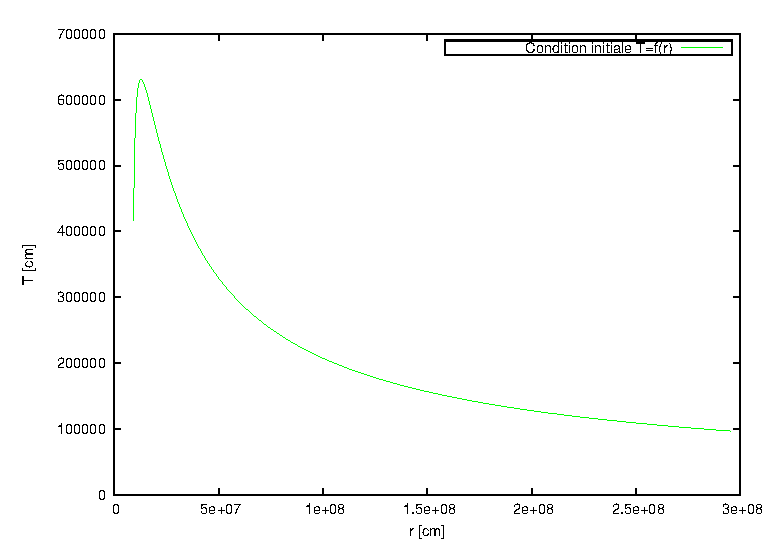
\includegraphics[scale=0.6]{ic_T.eps}
      \caption{Tracé de $T(r)$ à $t = 0$}\label{fig:CI_T}
   \end{minipage} \hfill
   \begin{minipage}[c]{.46\linewidth}
      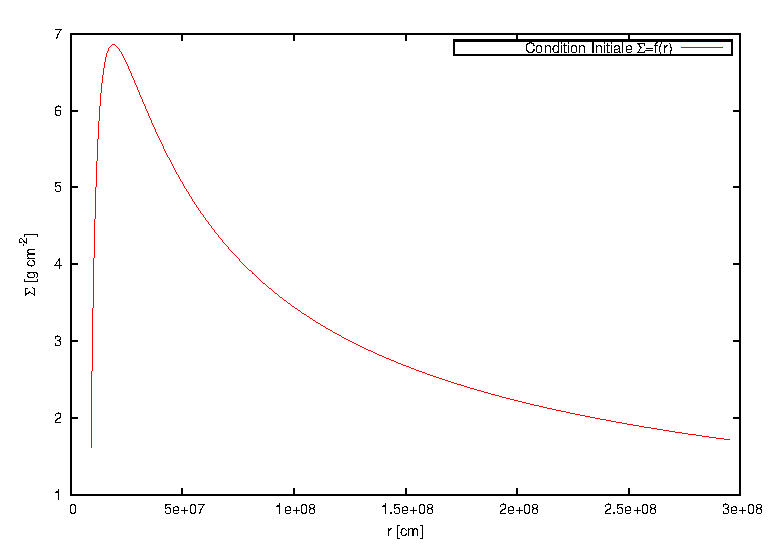
\includegraphics[scale=0.6]{ic_Sig.eps}
      \caption{Tracé de $\Sigma(r)$ à $t = 0$}\label{fig:CI_Sig}
   \end{minipage}
\end{figure} 

Nous pouvons voir sur les figures \ref{fig:CI_T} et \ref{fig:CI_Sig} les formes
de $T$ et $\Sigma$ en fonction de $r$ à l'instant initial.

Cela nous permet donc, à partir de l'utilisation du trinôme du second degré
explicité équation \eqref{eq:trinôme} de calculer la hauteur initiale du
disque. Dans le cas limite où s'expriment ces formules nous pouvons également
calculer le rapport $H/r$ à partir de la formule suivante : 

\begin{equation}
  \label{eq:H_r}
	\frac{H}{r} = 1.7 \times 10^{-2}\alpha^{- \frac{1}{10}} \left[ \frac{\dot{M}}{10^{16} \mbox{g} \mbox{s}^{-1}} \right]^{\frac{3}{20}} \left[ \frac{M}{M_\odot}\right]^{- \frac{3}{8}} \left[ \frac{r}{10^{10} \mathrm{cm}}\right]^{- \frac{1}{8}} f^{\frac{3}{5}}
\end{equation}
 
On peut alors comparer cette forme approximative avec la valeur simulée pour montrer que ces 
conditions initiales sont physiquement acceptables. Le tracé de cette courbe est effectué en figure \ref{fig:H_r}.

\begin{figure}
  \begin{center}
    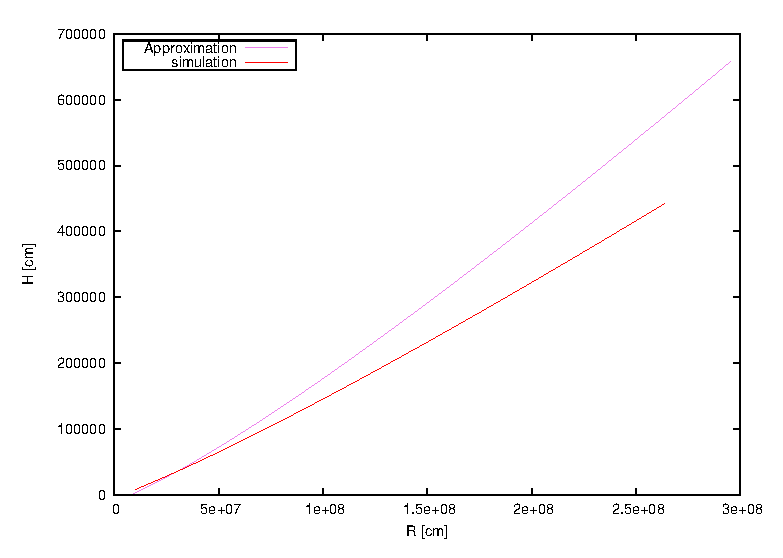
\includegraphics[]{ic_h.eps}
  \end{center}
  \caption{$H(r)$ à l'instant initial. La courbe rose est issue de la simulation, la courbe rouge est issue de l'équation \eqref{eq:H_r}}
  \label{fig:H_r}
\end{figure} 

Les deux formes étant toutes deux approximatives, on ne peut que comparer leurs
ordre de grandeurs qui sont compatibles. On supposera donc que les conditions
initiales sont physiquement raisonnables.